\documentclass[aspectratio=169,hyperref={pdfusetitle,pdfencoding=auto}]{beamer}
\usetheme{fub}

% Set \germantrue if the document is in German language
\newif\ifgerman
%\germanfalse
\germantrue
\ifgerman
  \def\babellanguage{ngerman}
  \def\polyglossialanguage{german}
  \def\biblatexsorting{de_DE}
\else
  \def\babellanguage{english}
  \def\polyglossialanguage{english}
  \def\biblatexsorting{en_US}

\fi

\usepackage{amsmath}
\usepackage{amssymb}
\usepackage{amsfonts}
\usepackage{amsthm}

% Font setup is tricky
\usefonttheme{professionalfonts}


\usepackage{iftex}
\ifPDFTeX
  \usepackage[utf8]{inputenc}
  \usepackage[T1]{fontenc}
  \usepackage{lmodern}
  \usepackage[\babellanguage]{babel}
\else
  \usepackage{unicode-math}
  \usepackage{fontspec}
  \setsansfont{CMU Sans Serif}
  \setmainfont{CMU Sans Serif}
  \setmonofont{CMU Typewriter Text}

  % Make it look more like CM Math
  % https://tex.stackexchange.com/q/140754/90407
  \setmathfont{Latin Modern Math}
  \setmathfont[range=\mathbb]{TeX Gyre Termes Math}

  % LM doesn't have the correct symbol for \setminus, workaround
  % https://tex.stackexchange.com/a/140343/90407
  \AtBeginDocument{\renewcommand{\setminus}{\mathbin{\backslash}}}

  \usepackage{polyglossia}
  \setdefaultlanguage{\polyglossialanguage}
\fi

\usepackage{microtype}
\usepackage{csquotes}

\usepackage{tikz}
\usetikzlibrary{positioning,shapes,fit}

\PassOptionsToPackage{hyphens}{url}

\makeatletter\def\blx@nowarnpolyglossia{}\makeatother
\usepackage[
  natbib=true,
  style=numeric,
  backend=biber,
  sorting=nty,
  sortlocale=\biblatexsorting,
  seconds=true,
  alldates=iso,
]{biblatex}
\addbibresource[]{./bibliography.bib}

% Display overview before each new section
\AtBeginSection[]
{
\begin{frame}
  \frametitle{Table of Contents}
  \tableofcontents[currentsection]
\end{frame}
}

\pgfdeclareimage[width=3cm]{logo}{./Fub-logo_svg.png}
\logo{\pgfuseimage{logo}}

\title{An example title}
\subtitle{With a longer subtitle}
\institute{Institute for Silly Walks}
\author{Leonard König\and Foo Bar}

\begin{document}

% Example content

\begin{frame}
  \titlepage
\end{frame}

\begin{frame}{Overview}
  \tableofcontents
\end{frame}


\section{Introduction}

\begin{frame}{Overview of topic}
This should give a neat introduction about what were speaking about.
\begin{itemize}
  \item Foo
  \item Bar \enquote{baz} buzz
  \item Buzz buss
  \item La li lo
\end{itemize}

\begin{figure}
\centering
\resizebox{!}{.3\textheight}{
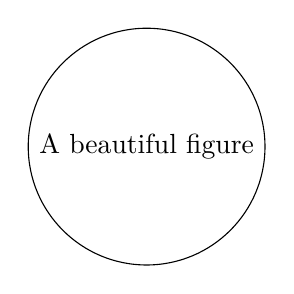
\begin{tikzpicture}[every node/.style={draw,circle}]
  \node {A beautiful figure};
\end{tikzpicture}
}
\caption{Caption of figure}
\end{figure}
\end{frame}


\subsection{Current Research}

\begin{frame}{An Example Research Method}
We now give overviews about current research methods.

\vfill
Note:
\begin{enumerate}
  \item These are bad because we don't like them
  \item If we need to back this up, we can do this~\cite{Author/2020}
  \item But if we don't want the references to clutter up
  \item We can keep \enquote{hide} these\nocite{Author/2020}
  \item They still show up in the bibliography
\end{enumerate}
\vfill
\pause
\alert{We want different methods!}
\end{frame}


\section{Going Forward}

\subsection{Our Stuff}

\begin{frame}{Idea: Think hard and visualize!}
\begin{itemize}[<+->]
  \item We can
  \item build lists
  \item incrementally
\end{itemize}
\vfill
Now for some example \enquote{animations}
\end{frame}

\begin{frame}{Probabilistic Graphical Models}
\begin{columns}
\begin{column}{.6\textwidth}
\begin{itemize}
  \item<1-3> Probability Variables \(X_1,\dotsc,X_5\) as nodes
  \item<2-3> Probabilistic Dependence: \(\Pr(X_2 \mid X_1) = p\)
  \item<3-3> Undirected Dependence: \(\Pr(X_2 \mid X_3) = p' = \Pr(X_3 \mid X_2)\)
  \item<only@4> Acyclic graph
  \item<only@5> Cycle
  \item<only@6> Bipartite Graph
\end{itemize}
\end{column}
\begin{column}{.4\textwidth}
\begin{figure}
\centering
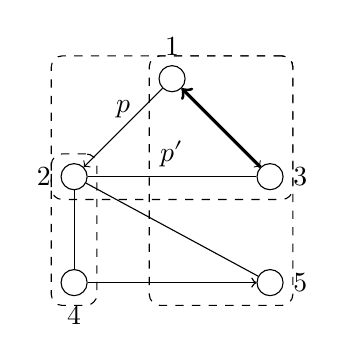
\begin{tikzpicture}
  \node[draw,circle,label={    1}                 ] (1) {};
  \node[draw,circle,label={180:2},below left =of 1] (2) {};
  \node[draw,circle,label={  0:3},below right=of 1] (3) {};
  \node[draw,circle,label={270:4},below      =of 2] (4) {};
  \node[draw,circle,label={  0:5},below      =of 3] (5) {};

  \visible<2->{
  \draw[->] (1) edge node[above] {$p$} (2);
  }
  \visible<3->{
  \draw[]   (2) edge node[above] {$p'$} (3);
  }
  \visible<4>{
  \draw[->] (1) -- (3);
  \draw[->] (2) -- (4) -- (5);
  }
  \visible<5>{
  \draw[->,line width=0.4mm] (3) -- (1);
  \draw[->] (2) -- (4) -- (5);
  \node[draw,rounded corners,dashed,fit=(1) (2) (3)] {};
  }
  \visible<6>{
  \draw (4) -- (5);
  \draw (2) -- (5);
  \node[draw,rounded corners,dashed,fit=(2) (4)] {};
  \node[draw,rounded corners,dashed,fit=(1) (3) (5)] {};
  }
\end{tikzpicture}
\caption{A PGM}
\end{figure}
\end{column}
\end{columns}
\end{frame}
\begin{frame}{Factor Graphs}
\begin{columns}
\begin{column}{.6\textwidth}
Factoring graphs reduces size
\begin{itemize}
  \item Every (maximal) Clique is replaced by a Factor
  \item<4-> No direct neighborships b/t Prob.\@ Variables
  \item<5-> Factor set \(F=\{a,b,c\}\).
  \item<5-> Factors hold prob.\@ distr.\@ about its neighbors, eg.\@
            c: \(\Pr(X_7\mid X_6) = \Pr(X_6 \mid X_7)\)
\end{itemize}
\end{column}
\begin{column}{.4\textwidth}
\begin{figure}
\centering
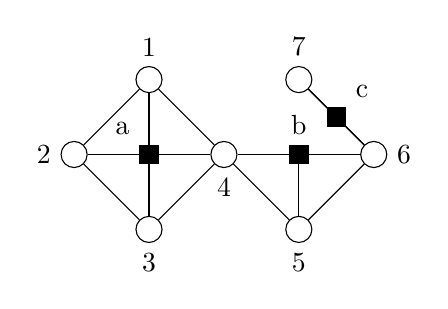
\begin{tikzpicture}[node distance=1cm]
  \node[draw,circle,label={    1}]                  (1) {};
  \node[draw,circle,label={180:2},below left =of 1] (2) {};
  \node[draw,circle,label={270:4},below right=of 1] (4) {};
  \node[draw,circle,label={270:3},below right=of 2] (3) {};
  \node[draw,circle,label={270:5},below right=of 4] (5) {};
  \node[draw,circle,label={  0:6},above right=of 5] (6) {};
  \node[draw,circle,label={ 90:7},above right=of 4] (7) {};

  \visible<1>{
  \draw (1) -- (2) -- (3) -- (4) -- (1);
  \draw (1) -- (3);
  }
  \visible<2->{
  \draw (1) -- (3) node[midway,fill,draw,label={135:a}] (a) {};
  \draw (2) -- (4);
  }
  \visible<1-2>{
  \draw (2) -- (4);
  \draw (4) -- (5) -- (6);
  \draw (6) -- (4);
  }
  \visible<3->{
  \draw (4) -- (6) node[midway,fill,draw,label={b}] (b) {};
  \draw (5) -- (b);
  }
  \visible<1-3>{
  \draw (6) -- (7);
  }
  \visible<4->{
  \draw (6) -- (7) node[midway,fill,draw,label={45:c}] (c) {};
  }
\end{tikzpicture}
\caption{\temporal<2-3>{Regular PGM}{\ldots}{Factor Graph}}
\end{figure}
\end{column}
\end{columns}
\end{frame}


\section{Conclusion}

\begin{frame}{Overview of what happened}
\begin{table}
\begin{tabular}{l|ccccc}
Features    & Approach 1 & Approach 2 & Approach 3 & Approach 4 & Approach 5 \\
\hline
Feature 1 & No  & No  & Yes     & N/A & Complex \\
Feature 2 & Yes & No  & Perhaps & Yes & Simple  \\
Feature 1 & No  & Yes & No      & No  & Complex 
\visible<2->{ \\ \hline
Rating    & $0.71$   & $0.55$ & $0.67$       & $0.66$ & $\mathbf{0.77}$      \\
Rating 2  & $\mathbf{0.29}$   & $0.11$ & $0.02$       & $0.05$ & $0.12$      
}
\end{tabular}
\caption{Comparison of approaches}
\end{table}
\end{frame}


\subsection{Evaluation \& Outlook}

\begin{frame}{Conclusion}
Results of the evaluation:
\begin{itemize}
  \item Our approach is better
  \item But things can be improved
  \item We could combine more ideas!
\end{itemize}
\end{frame}

\begin{frame}
\centering
\Huge Thanks for listening
\end{frame}

\begin{frame}[t,allowframebreaks,plain]
  \printbibliography
\end{frame}

% End example content

\end{document}
